%!TEX root = main.tex
\vspace{-.3cm}
\section{Our approach at work} % (fold)
\label{sec:case_studies}

In this section we discuss the case study gradually introduced in Figure~\ref{fig:arenarobot} and in Examples \ref{ex:controller}, \ref{ex:dtmc}, \ref{ex:environment}, \ref{ex:pomdp} and \ref{ex:formula} where we described the controller of the black robot, the environment model composed by white robots, the merged model as a \ac{POMDP}, and a possible target formula $\varphi_{avoid}$.
%We model the arena as a square matrix and the status of every robot as its position using coordinates. We are interested in evaluating the behaviour produced by our scheduler considering different objective properties.

%\marginpar{LTS}
%The controller is modeled by a \ac{LTS} $\mathcal{L}$ and, since we are assuming that the controller is aware of its own position inside the arena, we can model the state as the couple of coordinates given by its position $(x_0,y_0)$. In general we put every known information inside the controller's status. We let the robot moves in any direction from any position, that means that the controller can always choose to go towards any direction (north, south, east, west or to stand still) and the next state will depend on the chosen action and the starting state. 

%We denote the dimension of the arena with $DIM$ that represent the number of rows or column of the matrix. States and actions of the controller are defined as follows
%$$
%\begin{array}{rcl}
%	\mathcal{S}_\mathcal{L} &=& \left\{ (x,y)\ |\ x,y = 1,\dots,DIM \right\} \\
%	\mathcal{A}_\mathcal{L} &=& \left\{ north, south, east, west, here \right\}	\\
%\end{array}
%$$
%and $n$, $s$, $e$, $w$, $h$ are for, respectively, north, south, east, west and here. 

%To ease the next definitions we say that the function $next(x,y,a)$ returns the position that we obtain starting from $(x,y)$ and applying direction $a \in \mathcal{A}_{\mathcal{L}}$, assuming that moving towards a wall will not change the current position. The transition relation can be defined then as $T_{\mathcal{L}}(s,a)= step(s,a)$
%The transition relation $T_\mathcal{L}$ is built in order to move the position in the given action, e.g., $T((x,y),west) = (x-1,y)$ if $x > 0$, $T_\mathcal{L}((x,y),west) = (x,y)$ otherwise.

%\marginpar{MDP}
%The environment is modeled by $\mathcal{M}$, a \ac{MDP} that represents the probabilistic behaviour of two other robots. They can move independently in the four directions or stand still as the main robot. We assume that their movement are fully probabilistic with a uniform distribution over the reachable positions. The state of the environment \ac{MDP} $M$ is then represented by the coordinates of the two robots ($\mathcal{S}_\mathcal{M} = \mathcal{S}_\mathcal{L}^2)$, and it can receive any action from the controller ($\mathcal{A}_\mathcal{M} = \mathcal{A}_\mathcal{L}$).

%The transition relation $T_\mathcal{M}$ can always accept any action from the controller, since it is completely reactive, and the probabilistic behaviour that follows is not influenced, in this specific case study, by this choice. The next state distribution is obtained as the product of the distributions of both the robots of the environment. Then we can define $ T_{\mathcal{M}}((s_1,s_2),\cdot)(s_1',s_2') = p $ where $s_1'$ and $s_2'$ are positions directly reachable by one step starting from $s_1$ and $s_2$ respectively. The probability $p$ is the same per every reachable state of $\mathcal{M}$.

%\marginpar{POMDP}
%To merge together controller and environment into a product \ac{POMDP} $\mathcal{W}(\mathcal{L},\mathcal{M},\mathcal{O},Z)$ we need to define how the main robot perceive the others. We assume that the robot can perceive the presence of at least one robot in each of the four adjacent positions or in its own position, and that this perception is not affected by precision errors. Starting from a set of basic observations $ basic = \left\{north, south, east, west, here \right\} $ we obtain the set of possible observations as the power set $\mathcal{O} = \mathcal{P}(basic)$, indeed every basic observation can happen independently from the others.
%$$
%\begin{array}{rcl}
%	Z(s_0,s_1,s_2)(\{o_1,\dots,o_n\}) &=& 
%	\begin{cases}
%		1 \quad \text{if } s_1 \in next(s_0,o_i) \wedge s_2 \in next(s_0,o_i) \ \forall\ i \\
%		0 \quad \text{otherwise} \\
%	\end{cases} \\[.5cm]
%\end{array}
%$$

%$\mathcal{W}$ describe the whole system. We convert it into the explicit \ac{MDP} $\widehat{\mathcal{W}}$ and we export it to the \texttt{PRISM} model checker~\cite{KwiatkowskaNP11} to compute the minimum probability of satisfying a given objective formula $\varphi$. We obtain then a minimum probability for every state of the system, in this case one for each disposition of the robots.

%The problem of avoiding collisions with other robots as addressed with the following \ac{LTL} formula
%$$ \varphi_{avoid} = \neg\ collision \wedge \bigcirc\ \neg\ collision $$
%$$ Pmin=?[ G<=1 (! "collision")] $$
%where label $collision$ is defined as $\bigvee_{o \in \mathcal{O} : here \in o}o$.

We have run some experiments to compare the criterion we adopted with other possible approaches. The \textsc{avg} scheduler, the one we propose, chooses the action which maximize the minimum probability averaged over the belief probabilities. With scheduler \textsc{max} we consider to maximize the maximum minimum probability weighted again with belief probabilities. The \textsc{rnd} scheduler makes the robot move towards a uniformly random direction that is not already taken by another robot. \textsc{rpl} is the repulsive approach: the robot stands still until he perceive another robot, then it starts to move to the opposite direction, without keeping any memory of the past. \textsc{rpl} is defined for each pair state-observation.

We compare all the different approaches in a $5 \times 5$ arena with three robots, running $100$ simulations for $100$ steps for each case. Every run starts from a random initial state. The experiments results are shown in Figure~\ref{fig:exp} (left-hand side) where we measure the cumulate number of collisions over time, summing up over all the runs. 

Apart from some specific situation with the highest density of robots, the \textsc{avg} scheduler 
%manage to avoid collisions and it 
behaves generally better with respect to the other schedulers for collisions avoidance. It is worth noting that, the higher is the arena, the lower is the density of robots inside it; then avoiding collisions becomes easier. The \textsc{max} scheduler turns out to be suitable only for some specific situations since it gets good performances with a high density of robots.
% but they decrease as the density decreases.

Keeping other robots under observation is another possible target that can be expressed with a \ac{LTL} formula in the following way:
\vspace{-.2cm}
$$ \varphi_{track} = \neg\ collision \wedge vision \wedge \bigcirc\ (\neg\ collision \wedge vision) $$

\vspace{-.2cm}
\noindent
where $vision$ is a label that stands for $\neg\ \varnothing$ meaning that the robot is perceiving ``nothing''. 
Results from simulations depicted in Figure~\ref{fig:exp} (right-hand side) are obtained with the same set up of the previous experiment, and show that the synthesized behaviour is such that the number of perceptions is maximized while the number of collisions is minimized. 
It is worth noting that, by considering closely the simulation it is possible to appreciate some counterintuitive movement pattern such as moving towards other robots:
%By watching closely to the simulation
%\marginpar{Come fanno a watch-arlo?}
%it is possible to notice some unintuitive movement pattern such as moving towards other robots: 
this behaviour is actually the one that maximize our target since the other robot is more likely to move away from its current position making room for the controlled robot and, at the same time, remaining in its sight with probability $1$.
\begin{figure}[htbp]
	\centering
	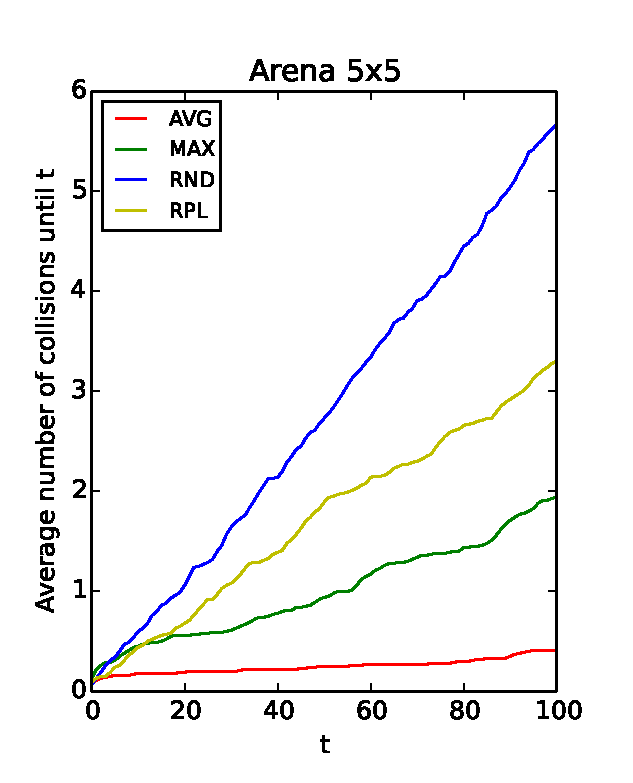
\includegraphics[width=0.42\textwidth]{figures/avoid_C0D5N3.eps}
	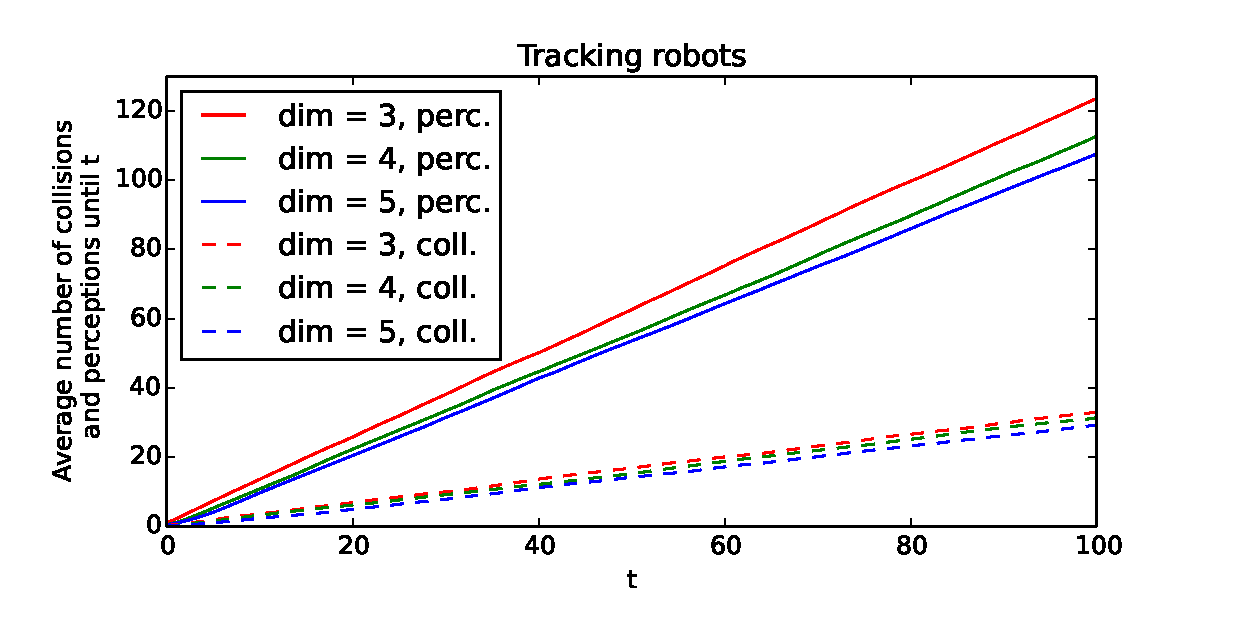
\includegraphics[width=0.42\textwidth]{figures/track_S0N3.eps}
	\caption{Collisions and perceptions with $\varphi_{track}$}
	\label{fig:exp}
\end{figure}

Simulations are written in python, code and data can be downloaded from  \url{http://dropproxy.com/f/BF7}\footnote{The actual code is also in a github repository but we do not report the link for the sake of anonymity.}.% \dots omissis \ldots %~\cite{github}.
%\marginpar{metterlo su dropbox se possibile o trovare un modo di anonimizzare github}
% section case_study (end)
